\documentclass{beamer}
\usetheme{ucl}

\newcommand\hmmax{0}
\newcommand\bmmax{0}

\usepackage{graphicx}%
\usepackage{multirow}%
\usepackage{amsmath,amssymb,amsfonts}%
%\usepackage{amsthm}%
\usepackage{stmaryrd}
\usepackage{mathrsfs}%
\usepackage[title]{appendix}%
\usepackage{xcolor}%
\usepackage{textcomp}%
\usepackage{manyfoot}%
\usepackage{booktabs}%
\usepackage{algorithm}%
\usepackage{algorithmicx}%
\usepackage{algpseudocode}%
\usepackage{listings}%
\usepackage{orcidlink}
\usepackage{comment}
%%%%
\usepackage{mathtools}  % For cases
%\usepackage{thm-restate}
%\usepackage{mathrsfs}
\usepackage[inline]{enumitem} %For enum*

\usepackage{mathbbol}
%\usepackage{tikz-cd} % For tikz art
%\usepackage{tikzit}
%\usepackage{ebproof}
\usepackage{bussproofs}
\usepackage{proof}


%%%%%%%%%%%%%%%%%%%%%%%%%%%%%%%%%%%%%%%%%%%%%%%%%%%%%%
%%%%%%%%%%%%%% Define the new environments here;
%\newenvironment{qparts}{\begin{enumerate}[{(}a{)}]}{\end{enumerate}}
% \def\endproofmark{$\Box$}
%\renewenvironment{proof}{\par{\bf Proof}:}{\hfill$\blacksquare$}

\newtheorem{defn}[theorem]{Definition}

\newtheorem{question}[theorem]{Question}
\newtheorem{remark}[theorem]{Remark}
\newtheorem{construction}[theorem]{Construction}
\newtheorem{observation}[theorem]{Observation}

%Make font sans-serif
\renewcommand{\familydefault}{\sfdefault}

%%%%%% Define commands here;

% Basic logic notation.
%\newcommand{\seq}{\triangleright}
\newcommand{\seq}{\Rightarrow }
\newcommand{\sequent}[2]{{#1} \seq {#2}}
\newcommand{\thmSequent}[2]{{#1} \vdash {#2}}

%%%%%%%%%%%%%%%%%%%%%%%%%%%%%%%%%%%%%%%%%
%       BeS
%%%%%%%%%%%%%%%%%%%%%%%%%%%%%%%%%%%%%%%%%
\newcommand{\base}[1]{\mathscr{#1}}
\newcommand{\baseB}{\base{B}}
\newcommand{\baseC}{\base{C}}
\newcommand{\baseD}{\base{D}}
\newcommand{\baseE}{\base{E}}
\newcommand{\baseF}{\base{F}}
\newcommand{\baseG}{\base{G}}
\newcommand{\baseH}{\base{H}}
\newcommand{\baseX}{\base{X}}
\newcommand{\baseY}{\base{Y}}
\newcommand{\baseZ}{\base{Z}}
\newcommand{\baseIMALL}{\base{N}}
\newcommand{\emptybase}{\varnothing}
\newcommand{\basis}[1]{\mathfrak{#1}}
% \newcommand{\at}[1]{\mathrm{#1}}
\newcommand{\at}[1]{{#1}}
\newcommand{\At}{\mathbb{A}}

%\newcommand{\baseGeq}{\succeq}
%\newcommand{\baseLeq}{\preceq}
\newcommand{\baseGeq}{\supseteq}
\newcommand{\baseLeq}{\subseteq}

\newcommand{\suppTor}[1]{\Vdash_{\!\!#1}}
% \newcommand{\supp}[1]{\Vdash_{\!\!#1}}
% \newcommand{\suppNew}[1]{\vDash_{\!#1}}
\newcommand{\suppNew}[1]{\Vdash^{*}_{\!#1}}
\newcommand{\entails}{\Vdash}
%\newcommand{\proves}[1]{\vdash_{\!\!#1}}
\newcommand{\proves}{\vdash}
\newcommand{\plus}{+}
\newcommand{\system}[1]{\mathsf{#1}}
\newcommand{\Atoms}{\set{A}}
\newcommand{\Formulas}{\set{F}}
\newcommand{\Bunches}{\set{B}}
\newcommand{\set}[1]{\mathbb{#1}}


%%%% ILL
\newcommand{\IPL}{IPL}
\newcommand{\IMLL}{IMLL}
\newcommand{\IMALL}{IMALL}
\newcommand{\ILL}{ILL}
%\newcommand{\provesIMALL}{\vdash_{\mathrm{IMALL}}}
%\newcommand{\provesILL}{\vdash_{\mathrm{ILL}}}
\newcommand{\provesILL}{\vdash}
\newcommand{\multiset}{\mathcal{M}}
\newcommand{\fmultiset}{\mathcal{M}_{\!{f}}}
\newcommand{\emptymultiset}{\varnothing}
\newcommand{\deriveBaseM}[1]{\vdash_{\!\!#1}}
\newcommand{\deriveBaseIPL}[1]{\vdash_{\!\!#1}^{\mathfrak{S}}}
\newcommand{\suppIPL}[1]{\Vdash_{ \!\!#1 }^{\!\!\mathfrak{S}}}
\newcommand{\suppM}[2]{\Vdash_{ \!\!#1 }^{ \!\!#2 }}
\newcommand{\suppIPLAlt}[2]{\Vvdash_{ \!\!#1 }^{ \!\!#2 }}
\newcommand{\suppMAlt}[2]{\Vvdash_{ \!\!#1 }^{ \!\!#2 }}
\newcommand{\suppL}[3]{\Vdash_{ \!\!#1 }^{{ \!\!#2 }\ctxt\hspace*{0.08cm}{ \!\!#3 }}}
%\newcommand{\IMALLformula}{\mathsf{Form}}
\newcommand{\ILLformula}{\mathsf{Form}}
\newcommand{\mand}{\otimes}
\newcommand{\mtop}{1}
\newcommand{\mto}{\multimap}
\newcommand{\aand}{\mathbin{\&}}
\newcommand{\aor}{\oplus}
\newcommand{\abot}{0}
\newcommand{\msetunion}{,}
\newcommand{\bang}{\mathop{!}}
\newcommand{\makeMultiset}[1]{\{#1\}}
\newcommand{\flatIMALL}[1]{{#1}^{\flat}}
\newcommand{\flatILL}[1]{{#1}^{\flat}}
\newcommand{\deflatIMALL}[1]{{#1}^{\natural}}
\newcommand{\deflatILL}[1]{{#1}^{\natural}}
\newcommand{\openaddrule}{\{}
\newcommand{\closeaddrule}{\}}
\newcommand{\Closeaddrule}[2]{\}^{#2}_{#1}}
\newcommand{\extAt}{\widetilde{\At}}
\DeclareMathSymbol{\fatcomma}{\mathrel}{bbold}{\lq\,}
%\newcommand{\lbang}{\mathop{!}}
\newcommand{\ctxt}{;}
\newcommand{\iplill}[1]{(#1)^\star}
\newcommand{\illipl}[1]{(#1)_\star}



\setbeamersize{description width=2em}
%%% Remove nav symbols (and shift any logo down to corner)
\setbeamertemplate{navigation symbols}{\vspace{-2ex}}
\setbeamertemplate{footline}[author title date]
\setbeamercolor{banner}{bg=darkpurple}
\useinnertheme{blockborder}

\graphicspath{{./images/} }
\title[P-tS for ILL]{Base-extension semantics for Intuitionistic Linear Logic}
%\author{\texorpdfstring{Yll Buzoku\newline\url{y.buzoku@ucl.ac.uk}}{https://www.homepages.ucl.ac.uk/~zcapybu/}}
\author{Yll Buzoku}
\institute[UCL]{%
  Department of Computer Science \\ %
  University College London
}
\date{May 9, 2023}

\AtBeginSection[]
{
  \begin{frame}
    \frametitle{Presentation root directory}
    \tableofcontents[currentsection]
  \end{frame}
}

\begin{document}
%%%%%%%%%%%%%%%%%%%%%%%%%%%%%%%%%%%%%%%%%%%%%%%%%%%%%%%%
%%%%%%%%%%%%%%%%%%%%%%%%%%%%%%%%%%%%%%%%%%%%%%%%%%%%%%%%
\begin{frame}
\titlepage
\end{frame}
%%%%%%%%%%%%%%%%%%%%%%%%%%%%%%%%%%%%%%%%%%%%%%%%%%%%%%%%
%%%%%%%%%%%%%%%%%%%%%%%%%%%%%%%%%%%%%%%%%%%%%%%%%%%%%%%%
\section*{Goals for this presentation}
\begin{frame}{Goals for this talk}
\begin{itemize}[label={-}]
\item To introduce Intuitionistic Linear Logic and a natural deduction system for it.
\item Present a Base-extension semantics for Intuitionistic Linear Logic.
\item Talk about some of the difficulties involved the process of developing such a semantics.
\pause
\item Is Tammy really a fox?
\end{itemize}
\end{frame}
%%%%%%%%%%%%%%%%%%%%%%%%%%%%%%%%%%%%%%%%%%%%%%%%%%%%%%%%
%%%%%%%%%%%%%%%%%%%%%%%%%%%%%%%%%%%%%%%%%%%%%%%%%%%%%%%%
\begin{frame}{Presentation root directory}
\tableofcontents
\end{frame}
%%%%%%%%%%%%%%%%%%%%%%%%%%%%%%%%%%%%%%%%%%%%%%%%%%%%%%%%
%%%%%%%%%%%%%%%%%%%%%%%%%%%%%%%%%%%%%%%%%%%%%%%%%%%%%%%%
\section*{????}
\begin{frame}\frametitle{Some Terminology} 
	\begin{defn}[Region]
	  Given a topological space $X$, a region is a non-empty, connected, open subset of $X$. The closure of a region is called a closed region. 
	\end{defn}
	\pause
	For the following definitions, let $f:U\subseteq \mathbb{C} \rightarrow \mathbb{C}$, where $U$ is a region.
	\begin{defn}[Holomorphic]
	A function $f$ is said to be \emph{holomorphic} if it differentiable at all points $z \in U$.
	\end{defn}
\end{frame}
%%%%%%%%%%%%%%%%%%%%%%%%%%%%%%%%%%%%%%%%%%%%%%%%%%%%%%%%
%%%%%%%%%%%%%%%%%%%%%%%%%%%%%%%%%%%%%%%%%%%%%%%%%%%%%%%%
\section{Overview of Intuitionistic Linear Logic}
\begin{frame}{Notation}
	\begin{itemize}[label={-}]
		\item $\At$ represents a fixed, countably infinite set of propositional atoms. 
		\item Lower case latin letters represent propositional atoms 
		\item Upper case latin letters represent finite multisets of propositional atoms. 
		\item The empty multiset is denoted $\emptymultiset$. 
		\item The sum of two multisets $\at{P}$ and $\at{Q}$ is denoted $\at{P},\at{Q}$. 
		\item Lower case greek letters represent ILL formulas.
		\item Upper case greek letters represent ILL finite multisets thereof. 
		\item Atomic multiset is taken to mean multiset of propositional atoms.
	\end{itemize}
\end{frame}
%%%%%%%%%%%%%%%%%%%%%%%%%%%%%%%%%%%%%%%%%%%%%%%%%%%%%%%%
\begin{frame}{A natural deduction system for ILL}
\begin{center}
\noindent\begin{minipage}{0.47\textwidth}\scriptsize
\begin{prooftree}
  \def\ScoreOverhang{0.5pt}
  	\AxiomC{}
  	\RightLabel{Ax}
  	\UnaryInfC{$\varphi\proves\varphi$}
\end{prooftree}
\end{minipage}
\vspace{2pt}
\noindent\begin{minipage}{0.47\textwidth}\scriptsize
	\begin{prooftree}
  	\def\ScoreOverhang{0.5pt}
  		\AxiomC{$\Gamma,\varphi \proves \psi$}
  		\RightLabel{$\mto$-I}
  		\UnaryInfC{$\Gamma \proves \varphi \mto \psi$}
	\end{prooftree}
	\begin{prooftree}
	\def\ScoreOverhang{0.5pt}
		\AxiomC{$\Gamma \proves \varphi$}
		\AxiomC{$\Delta \proves \psi$}
		\RightLabel{$\mand$-I}
		\BinaryInfC{$\Gamma,\Delta \proves \varphi\mand\psi$}
	\end{prooftree}
	\begin{prooftree}
	\def\ScoreOverhang{0.5pt}
		\AxiomC{}
		\RightLabel{$\mtop$-I}
		\UnaryInfC{$\proves \mtop$}
	\end{prooftree}
	\begin{prooftree}
	\def\ScoreOverhang{0.5pt}
		\AxiomC{$\Gamma \proves \varphi$}
		\AxiomC{$\Gamma \proves \psi$}
		\RightLabel{$\aand$-I}
		\BinaryInfC{$\Gamma \proves \varphi \aand \psi$}
	\end{prooftree}
	\begin{prooftree}
	\def\ScoreOverhang{0.5pt}
		\AxiomC{$\Gamma \proves \varphi_i$}
		\RightLabel{$\aor$-$\text{I}_i$}
		\UnaryInfC{$\Gamma \proves \varphi_0 \aor \varphi_1$}
	\end{prooftree}
	\begin{prooftree}
	\def\ScoreOverhang{0.5pt}
		\AxiomC{No $\abot$ intro rule}
	\end{prooftree}
\end{minipage}%%%%%%%%%%%%%%%%%%%%%%%%%%%%%%%%
\begin{minipage}{0.47\textwidth}\scriptsize
	\begin{prooftree}
  	\def\ScoreOverhang{0.5pt}
  		\AxiomC{$\Gamma \proves \varphi \mto \psi$}
  		\AxiomC{$\Delta \proves \varphi$}
  		\RightLabel{$\mto$-E}
  		\BinaryInfC{$\Gamma,\Delta \proves \psi$}
	\end{prooftree}
	\begin{prooftree}
	\def\ScoreOverhang{0.5pt}
		\AxiomC{$\Gamma \proves \varphi\mand\psi$}
		\AxiomC{$\Delta, \varphi, \psi \proves \chi$}
		\RightLabel{$\mand$-E}
		\BinaryInfC{$\Gamma, \Delta \proves \chi$}
	\end{prooftree}
	\begin{prooftree}
	\def\ScoreOverhang{0.5pt}
		\AxiomC{$\Gamma \proves \varphi$}
		\AxiomC{$\Delta \proves \mtop$}
		\RightLabel{$\mtop$-E}
		\BinaryInfC{$\Gamma,\Delta \proves \varphi$}
	\end{prooftree}
	\begin{prooftree}
	\def\ScoreOverhang{0.5pt}
		\AxiomC{$\Gamma \proves \varphi_0 \aand \varphi_1$}
		\RightLabel{$\aand$-$\text{E}_i$}
		\UnaryInfC{$\Gamma \proves \varphi_i$}
	\end{prooftree}
	\begin{prooftree}
	\def\ScoreOverhang{0.5pt}
		\AxiomC{$\Gamma \proves \varphi \aor \psi$}
		\AxiomC{$\Delta,\varphi \proves \chi$}
		\AxiomC{$\Delta,\psi \proves \chi$}
		\RightLabel{$\aor$-E}
		\TrinaryInfC{$\Gamma, \Delta \proves \chi$}
	\end{prooftree}
	\begin{prooftree}
	\def\ScoreOverhang{0.5pt}
		\AxiomC{$\Gamma \proves \abot$}
		\RightLabel{$\abot$-E}
		\UnaryInfC{$\Gamma \proves \varphi$}
	\end{prooftree}
\end{minipage}
\end{center}
\end{frame}
%%%%%%%%%%%%%%%%%%%%%%%%%%%%%%%%%%%%%%%%%%%%%%%%%%%%%%%%
\begin{frame}{A natural deduction system for ILL (cont.)}
\begin{center}
\begin{minipage}{0.75\textwidth}\scriptsize
	\begin{prooftree}
		\def\ScoreOverhang{0.5pt}
			\AxiomC{$\Gamma_1 \provesILL \bang\psi_1$}
			\AxiomC{$\ldots$}
			\AxiomC{$\Gamma_n \provesILL \bang\psi_n$}
			\AxiomC{$\bang\psi_1,\ldots, \bang\psi_n \provesILL \varphi$}
			\RightLabel{$\bang$-Promotion}
			\QuaternaryInfC{$\Gamma_1, \ldots,\Gamma_n \provesILL \bang\varphi$}
	\end{prooftree}
	\begin{prooftree}
		\def\ScoreOverhang{0.5pt}
			\AxiomC{$\Gamma \provesILL \bang\varphi$}
			\AxiomC{$\Delta, \varphi \provesILL \psi$}
			\RightLabel{$\bang$-Dereliction}
			\BinaryInfC{$\Gamma, \Delta\provesILL \psi$}
	\end{prooftree}
	\begin{prooftree}
		\def\ScoreOverhang{0.5pt}
			\AxiomC{$\Gamma \provesILL \bang\varphi$}
			\AxiomC{$\Delta \provesILL \psi$}
			\RightLabel{$\bang$-Weakening}
			\BinaryInfC{$\Gamma, \Delta\provesILL \psi$}
	\end{prooftree}
	\begin{prooftree}
		\def\ScoreOverhang{0.5pt}
			\AxiomC{$\Gamma \provesILL \bang\varphi$}
			\AxiomC{$\Delta,\bang\varphi,\bang\varphi \provesILL \psi$}
			\RightLabel{$\bang$-Contraction}
			\BinaryInfC{$\Gamma, \Delta\provesILL \psi$}
	\end{prooftree}
\end{minipage}
\end{center}
\end{frame}
%%%%%%%%%%%%%%%%%%%%%%%%%%%%%%%%%%%%%%%%%%%%%%%%%%%%%%%%
\begin{frame}{What is the general form of an inference figure?}
	\pause
	\begin{prooftree}
		\def\ScoreOverhang{0.5pt}
			\AxiomC{$\Gamma \proves \varphi$}
			\AxiomC{$\Delta \proves \psi$}
			\RightLabel{$\mand$-I}
			\BinaryInfC{$\Gamma,\Delta \proves \varphi\mand\psi$}
	\end{prooftree}
\end{frame}
%%%%%%%%%%%%%%%%%%%%%%%%%%%%%%%%%%%%%%%%%%%%%%%%%%%%%%%%
\begin{frame}{What is the general form of an inference figure?}
	\begin{prooftree}
		\def\ScoreOverhang{0.5pt}
			\AxiomC{$\Gamma \proves \varphi$}
			\AxiomC{$\Gamma \proves \psi$}
			\RightLabel{$\aand$-I}
			\BinaryInfC{$\Gamma \proves \varphi \aand \psi$}
		\end{prooftree}
\end{frame}
%%%%%%%%%%%%%%%%%%%%%%%%%%%%%%%%%%%%%%%%%%%%%%%%%%%%%%%%
\begin{frame}[b]{What is the general form of an inference figure?}
	\pause
	\begin{minipage}{0.47\textwidth}\scriptsize
		\begin{prooftree}
			\AxiomC{$\Gamma_1 \proves \varphi_1$}
			\AxiomC{$\dots$}
			\AxiomC{$\Gamma_n \proves \varphi_n$}
			\TrinaryInfC{$\Gamma_1 \dots \Gamma_n \proves \psi$}
		\end{prooftree}
	\end{minipage}
	\begin{minipage}{0.47\textwidth}\scriptsize
		\begin{prooftree}
			\AxiomC{$\Gamma \proves \varphi_1$}
			\AxiomC{$\dots$}
			\AxiomC{$\Gamma \proves \varphi_n$}
			\dashedLine
			\TrinaryInfC{$\Gamma \proves \psi$}
		\end{prooftree}
	\end{minipage}
	\vspace{2cm}
	\pause
	\begin{prooftree}
		\def\ScoreOverhang{0.5pt}
			\AxiomC{$\Gamma \proves \varphi \aor \psi$}
			\AxiomC{$\Delta,\varphi \proves \chi$}
			\AxiomC{$\Delta,\psi \proves \chi$}
			\RightLabel{$\aor$-E}
			\TrinaryInfC{$\Gamma, \Delta \proves \chi$}
	\end{prooftree}
\end{frame}
%%%%%%%%%%%%%%%%%%%%%%%%%%%%%%%%%%%%%%%%%%%%%%%%%%%%%%%%
\begin{frame}{What is the general form of an inference figure?}
	\begin{prooftree}
		\def\ScoreOverhang{0.5pt}
			\AxiomC{$\Gamma \proves \varphi \aor \psi$}
			\AxiomC{$\Delta,\varphi \proves \chi$}
			\AxiomC{$\Delta,\psi \proves \chi$}
			\RightLabel{$\aor$-E}
			\TrinaryInfC{$\Gamma, \Delta \proves \chi$}
	\end{prooftree}
\end{frame}
%%%%%%%%%%%%%%%%%%%%%%%%%%%%%%%%%%%%%%%%%%%%%%%%%%%%%%%%
\begin{frame}{What is the general form of an inference figure?}
	\begin{prooftree}
		\def\ScoreOverhang{0.5pt}
			\AxiomC{$\Gamma \proves \varphi \aor \psi$}
			\AxiomC{$\Delta\,\openaddrule\varphi \proves \chi$}
			\AxiomC{$\psi \proves \chi\closeaddrule$}
			\RightLabel{$\aor$-E}
			\TrinaryInfC{$\Gamma, \Delta \proves \chi$}
	\end{prooftree}
\end{frame}
%%%%%%%%%%%%%%%%%%%%%%%%%%%%%%%%%%%%%%%%%%%%%%%%%%%%%%%%
\begin{frame}{What is the general form of an inference figure?}
	\begin{prooftree}
		\def\ScoreOverhang{0.5pt}
			\AxiomC{$\Gamma\,\openaddrule \emptymultiset\proves \varphi \aor \psi\closeaddrule$}
			\AxiomC{$\Delta\,\openaddrule\varphi \proves \chi$}
			\AxiomC{$\psi \proves \chi\closeaddrule$}
			\RightLabel{$\aor$-E}
			\TrinaryInfC{$\Gamma, \Delta \proves \chi$}
	\end{prooftree}
\end{frame}
%%%%%%%%%%%%%%%%%%%%%%%%%%%%%%%%%%%%%%%%%%%%%%%%%%%%%%%%
\begin{frame}{What is the general form of an inference figure?}
	\begin{prooftree}
		\def\ScoreOverhang{0.5pt}
			\AxiomC{$\Gamma\,\openaddrule \emptymultiset\proves \varphi \aor \psi\closeaddrule$}
			\AxiomC{$\Delta\,\openaddrule\varphi \proves \chi$}
			\AxiomC{$\psi \proves \chi\closeaddrule$}
			\RightLabel{$\aor$-E}
			\TrinaryInfC{$\Gamma, \Delta \proves \chi$}
	\end{prooftree}
\end{frame}
%%%%%%%%%%%%%%%%%%%%%%%%%%%%%%%%%%%%%%%%%%%%%%%%%%%%%%%%
\begin{frame}{What is the general form of an inference figure?}
	\begin{prooftree}
		\def\ScoreOverhang{0.5pt}
			\AxiomC{$\Gamma\, \openaddrule\emptymultiset\proves \varphi\closeaddrule$}
			\AxiomC{$\Delta\, \openaddrule\emptymultiset\proves \psi\closeaddrule$}
			\RightLabel{$\mand$-I}
			\BinaryInfC{$\Gamma,\Delta \proves \varphi\mand\psi$}
	\end{prooftree}
	\vspace{1cm}
	\begin{prooftree}
		\def\ScoreOverhang{0.5pt}
			\AxiomC{$\Gamma\,\openaddrule \emptymultiset\proves \varphi$}
			\AxiomC{$\emptymultiset \proves \psi\closeaddrule$}
			\RightLabel{$\aand$-I}
			\BinaryInfC{$\Gamma \proves \varphi \aand \psi$}
		\end{prooftree}
\end{frame}
%%%%%%%%%%%%%%%%%%%%%%%%%%%%%%%%%%%%%%%%%%%%%%%%%%%%%%%%
\begin{frame}{What is the general form of an inference figure?}
		\begin{prooftree}
			\AxiomC{$\dots$}
			\AxiomC{$\Gamma_i\hspace*{5pt}\openaddrule \Delta_{i_1}\proves \varphi_{i_1}$}
			\AxiomC{$\dots$}
			\AxiomC{$\Delta_{i_{l_i}}\proves \varphi_{i_{l_i}}\closeaddrule$}
			\AxiomC{$\dots$}
			\QuinaryInfC{$\Gamma_1 \dots \Gamma_n \proves \psi$}
		\end{prooftree}
\end{frame}
%%%%%%%%%%%%%%%%%%%%%%%%%%%%%%%%%%%%%%%%%%%%%%%%%%%%%%%%
\begin{frame}{What is the general form of an inference figure?}
	\pause
	Almost! What about:\newline
	\begin{prooftree}
		\def\ScoreOverhang{0.5pt}
			\AxiomC{$\Gamma_1 \provesILL \bang\psi_1$}
			\AxiomC{$\ldots$}
			\AxiomC{$\Gamma_n \provesILL \bang\psi_n$}
			\AxiomC{$\bang\psi_1,\ldots, \bang\psi_n \provesILL \varphi$}
			\RightLabel{$\bang$-Promotion}
			\QuaternaryInfC{$\Gamma_1, \ldots,\Gamma_n \provesILL \bang\varphi$}
	\end{prooftree}
\end{frame}
%%%%%%%%%%%%%%%%%%%%%%%%%%%%%%%%%%%%%%%%%%%%%%%%%%%%%%%%
\begin{frame}{What is the general form of an inference figure?}
	\begin{prooftree}
		\def\ScoreOverhang{0.5pt}
			\AxiomC{$\Gamma_1\, \openaddrule\emptymultiset\provesILL \bang\psi_1\closeaddrule$}
			\AxiomC{$\ldots$}
			\AxiomC{$\Gamma_n\, \openaddrule\emptymultiset\provesILL \bang\psi_n\closeaddrule$}
			\AxiomC{$\bang\psi_1,\ldots, \bang\psi_n \provesILL \varphi$}
			\RightLabel{$\bang$-Promotion}
			\QuaternaryInfC{$\Gamma_1, \ldots,\Gamma_n \provesILL \bang\varphi$}
	\end{prooftree}
\end{frame}
%%%%%%%%%%%%%%%%%%%%%%%%%%%%%%%%%%%%%%%%%%%%%%%%%%%%%%%%
%%%%%%%%%%%%%%%%%%%%%%%%%%%%%%%%%%%%%%%%%%%%%%%%%%%%%%%%
\section{Base-extension Semantics for ILL}
\begin{frame}{Substructural atomic derivability}
\begin{definition}
Basic rules take the following form: 
\[\openaddrule (\at{P}_{1_i} \seq \at{q}_{1_i})\closeaddrule^{l_1}_{i=1}, \dots, \openaddrule (\at{P}_{n_i} \seq \at{q}_{n_i})\closeaddrule^{l_n}_{i=1} \Rightarrow \at{r}\]
where 
\begin{itemize}
\item Each $P_i$ is an atomic multiset, called a premiss multiset.
\item Each $q_i$ and $r$ is an atomic proposition.
\item Each $(P_i \seq q_i)$ is a pair $(P_i, q_i)$ called an atomic sequent.
\item Each collection $\openaddrule (\at{P}_{i_1} \seq \at{q}_{i_1}), \dots, (\at{P}_{i_{l_i}} \seq \at{q}_{i_{l_i}})\closeaddrule$ is called an atomic box.
    \end{itemize}
\end{definition}
\end{frame}
%%%%%%%%%%%%%%%%%%%%%%%%%%%%%%%%%%%%%%%%%%%%%%%%%%%%%%%%
\begin{frame}{Substructural atomic derivability}
\begin{definition}[Basic derivability relation]
The relation of derivability in a base $\baseB$, is defined inductively as so:
\begin{itemize}
\item[Ref] $p \deriveBaseM{\baseB} p$
\item[App] Given that $(\openaddrule(\at{P}_{1_i} \seq \at{q}_{1_{i}})\Closeaddrule{i=1}{l_1},\dots,\openaddrule(\at{P}_{n_i} \seq \at{q}_{n_{i}}) \Closeaddrule{i=1}{l_n} \Rightarrow \at{r}) \in \baseB$ and atomic multisets $\at{C}_i$ such that the following hold:
        \[\at{C}_i, \at{P}_{i_j} \deriveBaseM{\baseB} \at{q}_{i_j} \text{ for all } i = 1,\dots, n \text{ and } j = 1,\dots,l_i\]
Then $\at{C}_{1},\dots,\at{C}_{n}\deriveBaseM{\baseB} r$. 
\end{itemize}
\end{definition}
\end{frame}
%%%%%%%%%%%%%%%%%%%%%%%%%%%%%%%%%%%%%%%%%%%%%%%%%%%%%%%%
\begin{frame}{Base-extension Semantics for ILL}
\begin{center}
\begin{itemize}
\item[(At)] $\suppM{\baseB}{\at{L}} \at{p}$ iff $\at{L} \deriveBaseM{\baseB} \at{p}$. 
\item[($\mand$)] $\suppM{\baseB}{\at{L}} \varphi \mand \psi$ iff for every $\baseC \baseGeq \baseB$, atomic multiset $\at{K}$, and atom $\at{p}$, if $\varphi\fatcomma\psi\suppM{\baseC}{\at{K}} \at{p}$ then $\suppM{\baseC}{\at{L},\at{K}} \at{p}$. 
        % 
\item[($\mtop$)] $\suppM{\baseB}{\at{L}} \mtop$ iff for every $\baseC \baseGeq \baseB$, atomic multiset $\at{K}$, and atom $\at{p}$, if $\suppM{\baseC}{\at{K}} \at{p}$, then $\suppM{\baseC}{\at{L},\at{K}} \at{p}$. 
        % 
\item[($\mto$)] $\suppM{\baseB}{\at{L}} \varphi \mto \psi$ iff $\varphi \suppM{\baseB}{\at{L}} \psi$. 
        % 
\end{itemize}
\end{center}
\hspace{0.5\textwidth}\vdots
\end{frame}
%%%%%%%%%%%%%%%%%%%%%%%%%%%%%%%%%%%%%%%%%%%%%%%%%%%%%%%%
\begin{frame}{Base-extension Semantics for ILL}
	\hspace{0.5\textwidth}\vdots
	\begin{center}
	\begin{itemize}
        \item[($\aand$)] $\suppM{\baseB}{L} \varphi \aand \psi$ iff $\suppM{\baseB}{L} \varphi$ and $\suppM{\baseB}{L} \psi$. 
        %
        \item[($\aor$)] 
        $\suppM{\baseB}{L} \varphi \aor \psi$ iff for every $\baseC \baseGeq \baseB$, atomic multiset $\at{K}$ and atom $p \in \At$ such that $\varphi \suppM{\baseC}{\at{K}} \at{p}$ and $\psi \suppM{\baseC}{\at{K}} \at{p}$ hold, then $\suppM{\baseC}{\at{L},\at{K}} \at{p}$. 
        %
        \item[($\abot$)] $\suppM{\baseB}{\at{L}} \abot$ iff $\suppM{\baseB}{\at{L}} \at{p}$, for all $\at{p} \in \At$.
	\end{itemize}
	\end{center}
	\hspace{0.5\textwidth}\vdots
	\end{frame}
%%%%%%%%%%%%%%%%%%%%%%%%%%%%%%%%%%%%%%%%%%%%%%%%%%%%%%%%
\begin{frame}{Base-extension Semantics for ILL}
	\hspace{0.5\textwidth}\vdots
	\begin{center}
	\begin{itemize}
        \item[$(\fatcomma$)] $\suppM{\baseB}{\at{L}}\Gamma\fatcomma\Delta$ iff there are atomic multisets $\at{K}$ and $\at{M}$ such that $L=K,M$ and that $\suppM{\baseB}{\at{K}}\Gamma$ and $\suppM{\baseB}{\at{M}}\Delta$.
        %
        \item[($\bang$)] $\suppM{\baseB}{L} \bang \varphi$ iff for any $\baseC$ such that $\baseC \baseGeq \baseB$, atomic multisets $K$ and any $\at{p} \in \At$, if for any $\baseD$ such that $\baseD\baseGeq\baseC$,\,(if $\suppM{\baseD}{\emptymultiset}\varphi$ then $\suppM{\baseD}{L}\at{p})$ then $\suppM{\baseC}{L,K}\at{p}$.
        %
        \item[(Inf)] For $\Gamma=\bang\Delta\fatcomma\Theta$ being a nonempty multiset, $\Gamma \suppM{\baseB}{L}\varphi$ iff for all $\baseC \baseGeq \baseB$, atomic multisets $\at{K}$, if $\suppM{\baseC}{\at{K}}\Theta$ and $\suppM{\baseC}{\emptymultiset}\Delta$ then $\suppM{\baseC}{L,K}\varphi$.
	\end{itemize}
	\end{center}
	\pause
	Note the clause for ($\bang$) could be written as:
	\begin{itemize}
		\item $\suppM{\baseB}{L} \bang \varphi$ iff for any $\baseC$ such that $\baseC \baseGeq \baseB$, atomic multisets $K$ and any $\at{p} \in \At$, if $\bang\varphi\suppM{\baseC}{K}\at{p}$ then $\suppM{\baseC}{L,K}\at{p}$.
	\end{itemize}
	\end{frame}
%%%%%%%%%%%%%%%%%%%%%%%%%%%%%%%%%%%%%%%%%%%%%%%%%%%%%%%%
\begin{frame}{Notes on $\suppM{\baseB}{\at{L}}$}
	\begin{itemize}
	\item The sequent $\langle\Gamma,\varphi\rangle$ is said to be valid if and only if $\Gamma\suppM{\emptybase}{\emptymultiset}\varphi$ holds.
	\pause
	\item We frequently write this as $\Gamma \suppM{}{}\varphi$.
	\end{itemize}
\end{frame}
%%%%%%%%%%%%%%%%%%%%%%%%%%%%%%%%%%%%%%%%%%%%%%%%%%%%%%%%
\begin{frame}{Notes on $\suppM{\baseB}{\at{L}}$}
\begin{itemize}
\item If $\suppM{\baseB}{\at{L}}\varphi$ then for all $\baseC \baseGeq \baseB$ we have $\suppM{\baseC}{\at{L}}\varphi$.
\vspace{5pt}
\item $\suppM{\baseB}{\at{L}}\varphi$  iff $\suppM{\baseB}{\at{L}}\varphi\mand\mtop$ iff $\suppM{\baseB}{\at{L}}\varphi\fatcomma\mtop$
\vspace{5pt}
\item $\Gamma \suppM{\baseB}{\at{L}}\varphi$ iff for all $\baseC \baseGeq \baseB$ and atomic multisets $\at{K}$,\, $\suppM{\baseC}{\at{K}}\Gamma$ implies $\suppM{\baseC}{\at{L},\at{K}}\varphi$. 
%\vspace{5pt}
%\item $\suppM{\baseB}{\at{L}}\varphi$ iff for all $\baseC \baseGeq \baseB$ and atomic multisets $\at{K}$ and atoms $p$,\, $\varphi\suppM{\baseC}{K}p$ implies $\suppM{\baseC}{L,K}p$. 
\end{itemize}
\end{frame}
%%%%%%%%%%%%%%%%%%%%%%%%%%%%%%%%%%%%%%%%%%%%%%%%%%%%%%%%
\begin{frame}{Soundness}
	\begin{theorem}[Soundness]
		\centering
		If $\Gamma\proves\varphi$ then $\Gamma\suppM{}{}\varphi$
	\end{theorem}
	\pause
	\begin{itemize}
		\item The strategy is to show every rule of the natural deduction system presented previously is semantically expressible.
		\item This suffices by induction to prove this theorem as now we can encode any deduction into a series of semantic proofs.
	\end{itemize}
\end{frame}
\begin{frame}
	\begin{example}
		\centering
		If $\Gamma\fatcomma\varphi \suppM{}{}\psi$ then $\Gamma\suppM{}{}\varphi\mto\psi$.
	\end{example}
	\begin{proof}
		\begin{itemize}
			\item The hypothesis iff all bases $\baseB$ and atomic multisets $M=K,L$ where $\suppM{\baseB}{K}\varphi$ and $\suppM{\baseB}{L}\Gamma$ implies $\suppM{\baseB}{M}\psi$.
			\pause
			\item Monotonicity gives that this holds in all $\baseC \baseGeq \baseB$.
			\pause
			\item Thus we have that $\varphi\suppM{\baseB}{L}\psi$.
			\pause
			\item $\suppM{\baseB}{L}\varphi\mto\psi$ if and only if $\varphi\suppM{\baseB}{L}\psi$.
			\pause
			\item So we obtain that $\suppM{\baseB}{L}\varphi\mto\psi$ and thus $\Gamma\suppM{}{}\varphi\mto\psi$
		\end{itemize}
	\end{proof}
\end{frame}
%%%%%%%%%%%%%%%%%%%%%%%%%%%%%%%%%%%%%%%%%%%%%%%%%%%%%%%%
\begin{frame}{Completeness}
	\begin{theorem}[Completeness]
		\centering
		If $\Gamma\suppM{}{}\varphi$ then $\Gamma\proves\varphi$.
	\end{theorem}
	\pause
	\begin{itemize}
		\item Define two functions $\flatILL{(\cdot)}:\ILLformula \rightarrow \At$ and $\deflatILL{(\cdot)}:\At\rightarrow\ILLformula$.
		\item Show that any valid sequent remains valid when ``atomised".
		\item Construct a base $\baseILL$ whose rules simulate the natural deduction rules of ILL.
		\item Show that every derivation in this simulation base is equivalent to a corresponding derivation in ILL.
		\item Show we can go from a valid atomic derivation to a derivation in ILL.
	\end{itemize}
\end{frame}
%%%%%%%%%%%%%%%%%%%%%%%%%%%%%%%%%%%%%%%%%%%%%%%%%%%%%%%%
\section{Including the exponential}
\begin{frame}{What of the exponential?}
\begin{center}
\emph{The exponential is hard...}
\linebreak
\newline
\vspace{0.5cm}
\pause
\emph{But I finally got it!}
\end{center}
\end{frame}
%%%%%%%%%%%%%%%%%%%%%%%%%%%%%%%%%%%%%%%%%%%%%%%%%%%%%%%%
\begin{frame}{Why was it so hard?}
	\begin{center}
		\begin{minipage}{\textwidth}\scriptsize
			\begin{prooftree}
				\def\ScoreOverhang{0.5pt}
					\AxiomC{$\Gamma_1 \provesILL \bang\psi_1$}
					\AxiomC{$\ldots$}
					\AxiomC{$\Gamma_n \provesILL \bang\psi_n$}
					\AxiomC{$\bang\psi_1,\ldots, \bang\psi_n \provesILL \varphi$}
					\RightLabel{$\bang$-Promotion}
					\QuaternaryInfC{$\Gamma_1, \ldots,\Gamma_n \provesILL \bang\varphi$}
			\end{prooftree}
			\begin{prooftree}
				\def\ScoreOverhang{0.5pt}
					\AxiomC{$\Gamma \provesILL \bang\varphi$}
					\AxiomC{$\Delta, \varphi \provesILL \psi$}
					\RightLabel{$\bang$-Dereliction}
					\BinaryInfC{$\Gamma, \Delta\provesILL \psi$}
			\end{prooftree}
			\begin{prooftree}
				\def\ScoreOverhang{0.5pt}
					\AxiomC{$\Gamma \provesILL \bang\varphi$}
					\AxiomC{$\Delta \provesILL \psi$}
					\RightLabel{$\bang$-Weakening}
					\BinaryInfC{$\Gamma, \Delta\provesILL \psi$}
			\end{prooftree}
			\begin{prooftree}
				\def\ScoreOverhang{0.5pt}
					\AxiomC{$\Gamma \provesILL \bang\varphi$}
					\AxiomC{$\Delta,\bang\varphi,\bang\varphi \provesILL \psi$}
					\RightLabel{$\bang$-Contraction}
					\BinaryInfC{$\Gamma, \Delta\provesILL \psi$}
			\end{prooftree}
		\end{minipage}
	\end{center}
\end{frame}
%%%%%%%%%%%%%%%%%%%%%%%%%%%%%%%%%%%%%%%%%%%%%%%%%%%%%%%%
%\begin{frame}{What of the exponential?}
%	\begin{itemize}
%	\item All "structural" aspects of the exponential are on the \emph{left} hand side.
%	\pause
%	\item The exponential right rule, still depends fully on the structure of the left hand side.
%	\pause
%	\item None of these rules are invertible, so none are particularly nice candidates for giving a definition. 
%	\end{itemize}
%	\pause
%	However, this means that to pinpoint the behaviour of the exponential, we need to pinpoint something about the resources which can be used to support it! 
%\end{frame}
%%%%%%%%%%%%%%%%%%%%%%%%%%%%%%%%%%%%%%%%%%%%%%%%%%%%%%%%
\begin{frame}{Why was it so hard?}
	\begin{prooftree}
		\AxiomC{$\bang\psi \provesILL \bang\psi$}
		\AxiomC{$\bang\psi \provesILL \varphi$}
		\BinaryInfC{$\bang\psi\provesILL \bang\varphi$}
	\end{prooftree}
\end{frame}
%%%%%%%%%%%%%%%%%%%%%%%%%%%%%%%%%%%%%%%%%%%%%%%%%%%%%%%%
\begin{frame}{What do we have now?}
	\begin{center}
		\begin{itemize}
			\item[($\bang$)] $\suppM{\baseB}{L} \bang \varphi$ iff for any $\baseC$ such that $\baseC \baseGeq \baseB$, atomic multisets $K$ and any $\at{p} \in \At$, if $\bang\varphi\suppM{\baseC}{K}p$ then $\suppM{\baseC}{L,K}\at{p}$.
			%
			\vspace{1cm}
			%
			\item[(Inf)] For $\Gamma=\bang\Delta\fatcomma\Theta$ being a nonempty multiset, $\Gamma \suppM{\baseB}{L}\varphi$ iff for all $\baseC \baseGeq \baseB$, atomic multisets $\at{K}$, if $\suppM{\baseC}{\at{K}}\Theta$ and $\suppM{\baseC}{\emptymultiset}\Delta$ then $\suppM{\baseC}{L,K}\varphi$.
		\end{itemize}
	\end{center}
\end{frame}
%%%%%%%%%%%%%%%%%%%%%%%%%%%%%%%%%%%%%%%%%%%%%%%%%%%%%%%%
\begin{frame}{What do we know?}
	An important identity from Intuitionistic Linear Logic:
	\begin{itemize}
	\item $\bang\varphi \suppM{}{} \varphi \mand \ldots \mand \varphi$
	\end{itemize}
\end{frame}
%%%%%%%%%%%%%%%%%%%%%%%%%%%%%%%%%%%%%%%%%%%%%%%%%%%%%%%%
\begin{frame}{Expanding what we know}
	\begin{center}
	\begin{align*}
	&\bang\varphi \suppM{}{} \varphi \mand \ldots \mand \varphi \text{ iff } \\
	&\text{ for all bases } \baseB \text{ and atomic multisets } \at{L} \text{, such that } \suppM{\baseB}{\at{L}} \bang\varphi \text{ then } \\ 
	&\suppM{\baseB}{\at{L}} \varphi \mand \ldots \mand \varphi
	\end{align*}
	\end{center}
\end{frame}
%%%%%%%%%%%%%%%%%%%%%%%%%%%%%%%%%%%%%%%%%%%%%%%%%%%%%%%%
%%%%%%%%%%%%%%%%%%%%%%%%%%%%%%%%%%%%%%%%%%%%%%%%%%%%%%%%
\begin{frame}{Expanding what we know}
	\begin{center}
	\begin{itemize}
	\item So when does $\suppM{\baseB}{\at{L}} \varphi \mand \ldots \mand \varphi$ hold?
	\end{itemize}
	\end{center}
\end{frame}
%%%%%%%%%%%%%%%%%%%%%%%%%%%%%%%%%%%%%%%%%%%%%%%%%%%%%%%%
\begin{frame}{Expanding what we know}
	\begin{center}
	Considering the case when $\varphi = \at{p}$ for simplicity we get the following:
	\begin{itemize}
	\pause
	\item Given a base $\baseB$ such that $\deriveBaseM{\baseB}\at{p}$ and $\at{L}=\emptymultiset$.
	\pause
	\item Then we have that $\suppM{\baseB}{\at{L}}\at{p} \mand \ldots \mand \at{p}$.
	\pause
	\item Examples of such bases:
	\begin{itemize}
		\item $\baseB = \{ (\Rightarrow p)\}$
		\item $\baseB = \{(\Rightarrow q),\, (q\Rightarrow p) \}$
		%\item $\baseB = \{\at{r},\, \}$ and $\at{L}=\[\at{r}\]$
	\end{itemize}
	\pause
	\end{itemize} 
	\vspace{10pt}
	Note that if $\at{L}$ were non-empty then all of the atoms in $L$, call them $r_i$, would have to be derivable purely from $\baseB$.
	\end{center}
\end{frame}
%%%%%%%%%%%%%%%%%%%%%%%%%%%%%%%%%%%%%%%%%%%%%%%%%%%%%%%%
\begin{frame}{Expanding what we know}
	\begin{center}
	\noindent
	\emph{Inferring from $\bang \varphi$ should imply that $\suppM{\baseB}{\emptymultiset}\varphi$.}
	\end{center}
\end{frame}
%%%%%%%%%%%%%%%%%%%%%%%%%%%%%%%%%%%%%%%%%%%%%%%%%%%%%%%%
\begin{frame}{Alternative approach}
\begin{center}
\begin{itemize}
\begin{prooftree}
\AxiomC{$[P_1;C_1]$}
\noLine
\UnaryInfC{$\vdots$}
\noLine
\UnaryInfC{$q_1$}
\AxiomC{$\dots$}
\AxiomC{$[P_n;C_n]$}
\noLine
\UnaryInfC{$\vdots$}
\noLine
\UnaryInfC{$q_n$}
\RightLabel{$\mathcal{R}$}
\TrinaryInfC{$r$}
\end{prooftree}
\end{itemize}
\end{center}
\end{frame}
%%%%%%%%%%%%%%%%%%%%%%%%%%%%%%%%%%%%%%%%%%%%%%%%%%%%%%%%
\begin{frame}{Is Tammy really a fox?}
	\pause
	\centering
	\textbf{Maybe?}\linebreak
	\pause
	But I actually now think she is a Cat $\ldots$\linebreak
	\pause
	Specifically a symmetric monoidal cat!
\end{frame}
%%%%%%%%%%%%%%%%%%%%%%%%%%%%%%%%%%%%%%%%%%%%%%%%%%%%%%%%
\begin{frame}{Thank you!}
\begin{figure}
	\begin{center}
	  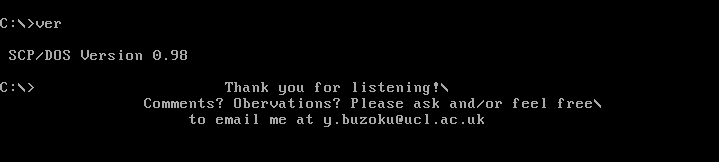
\includegraphics[width=\textwidth]{dosthanks2.png}
	  \caption{Thank you from DOS!\,:D}
	\end{center}
  \end{figure}
\end{frame}
%%%%%%%%%%%%%%%%%%%%%%%%%%%%%%%%%%%%%%%%%%%%%%%%%%%%%%%%
%\begin{frame}{Thank you!}
%\begin{center}
%Thank you for listening!

%Questions? Comments? Observations? Please ask and/or feel free to email me at \url{y.buzoku@ucl.ac.uk}.
%\end{center}
%\end{frame}
%%%%%%%%%%%%%%%%%%%%%%%%%%%%%%%%%%%%%%%%%%%%%%%%%%%%%%%%
\begin{frame}[allowframebreaks]
	\frametitle{References}
	\nocite{*}
	\bibliographystyle{amsalpha}
	\bibliography{./refs/refs.bib}
\end{frame}
%%%%%%%%%%%%%%%%%%%%%%%%%%%%%%%%%%%%%%%%%%%%%%%%%%%%%%%%
\end{document}
